\renewcommand{\leveltopI}{-15cm + \leveltop}
\renewcommand{\leveltopII}{-15cm + \leveltopI}
\renewcommand{\leveltopIII}{-15cm + \leveltopII}
\renewcommand{\leveltopIIII}{-15cm + \leveltopIII}
\renewcommand{\leveltopIIIII}{-15cm + \leveltopIIII}
\renewcommand{\leveltopIIIIII}{-15cm + \leveltopIIIII}
\renewcommand{\leveltopIIIIIII}{-15cm + \leveltopIIIIII}
\renewcommand{\leveltopIIIIIIII}{-15cm + \leveltopIIIIIII}
\renewcommand{\leveltopIIIIIIIII}{-15cm + \leveltopIIIIIIII}
\renewcommand{\leveltopIIIIIIIIII}{-15cm + \leveltopIIIIIIIII}
\renewcommand{\leveltopIIIIIIIIIII}{-15cm + \leveltopIIIIIIIIII}
\begin{tikzpicture}[scale=.2, anchor=south]
\begin{scope}[yshift=\leveltopI cm]
\matrix (line1) [column sep=1cm] {
\node[draw=black, rectangle split,  rectangle split parts=3] (sn0xd2f280){
\begin{tikzpicture}[scale=.2]
\node[circle, scale=0.75, fill] (tid0) at (3.75,1.5){};
\node[circle, scale=0.75, fill] (tid1) at (2.25,3){};
\node[circle, scale=0.75, fill] (tid3) at (0.75,4.5){};
\node[circle, scale=0.75, fill, red] (tid7) at (0.75,6){};
\draw[](tid3) -- (tid7);
\node[circle, scale=0.75, fill] (tid4) at (2.25,4.5){};
\node[circle, scale=0.75, fill] (tid5) at (3.75,4.5){};
\draw[](tid1) -- (tid3);
\draw[](tid1) -- (tid4);
\draw[](tid1) -- (tid5);
\node[circle, scale=0.75, fill] (tid2) at (6,3){};
\node[circle, scale=0.75, fill] (tid6) at (6,4.5){};
\node[circle, scale=0.75, fill] (tid8) at (5.25,6){};
\node[circle, scale=0.75, fill, red] (tid10) at (5.25,7.5){};
\draw[](tid8) -- (tid10);
\node[circle, scale=0.75, fill, red] (tid9) at (6.75,6){};
\draw[](tid6) -- (tid8);
\draw[](tid6) -- (tid9);
\draw[](tid2) -- (tid6);
\draw[](tid0) -- (tid1);
\draw[](tid0) -- (tid2);
\end{tikzpicture}
\nodepart{two}
\footnotesize{6.08445}
\nodepart{three}
\footnotesize{$33\:33\:33$}
};
 & 
\\
};
\end{scope}
\begin{scope}[yshift=\leveltopII cm]
\matrix (line2) [column sep=1cm] {
\node[draw=black, rectangle split,  rectangle split parts=3] (sn0xd31900){
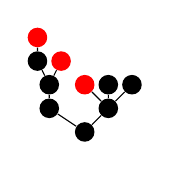
\begin{tikzpicture}[scale=.2]
\node[circle, scale=0.75, fill] (tid0) at (3.75,1.5){};
\node[circle, scale=0.75, fill] (tid1) at (1.5,3){};
\node[circle, scale=0.75, fill] (tid3) at (1.5,4.5){};
\node[circle, scale=0.75, fill] (tid7) at (0.75,6){};
\node[circle, scale=0.75, fill, red] (tid9) at (0.75,7.5){};
\draw[](tid7) -- (tid9);
\node[circle, scale=0.75, fill, red] (tid8) at (2.25,6){};
\draw[](tid3) -- (tid7);
\draw[](tid3) -- (tid8);
\draw[](tid1) -- (tid3);
\node[circle, scale=0.75, fill] (tid2) at (5.25,3){};
\node[circle, scale=0.75, fill, red] (tid4) at (3.75,4.5){};
\node[circle, scale=0.75, fill] (tid5) at (5.25,4.5){};
\node[circle, scale=0.75, fill] (tid6) at (6.75,4.5){};
\draw[](tid2) -- (tid4);
\draw[](tid2) -- (tid5);
\draw[](tid2) -- (tid6);
\draw[](tid0) -- (tid1);
\draw[](tid0) -- (tid2);
\end{tikzpicture}
\nodepart{two}
\footnotesize{5.81524}
\nodepart{three}
\footnotesize{$33\:33\:33$}
};
 & 
\node[draw=black, rectangle split,  rectangle split parts=3] (sn0xd2e850){
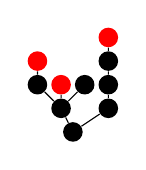
\begin{tikzpicture}[scale=.2]
\node[circle, scale=0.75, fill] (tid0) at (3,1.5){};
\node[circle, scale=0.75, fill] (tid1) at (2.25,3){};
\node[circle, scale=0.75, fill] (tid3) at (0.75,4.5){};
\node[circle, scale=0.75, fill, red] (tid7) at (0.75,6){};
\draw[](tid3) -- (tid7);
\node[circle, scale=0.75, fill, red] (tid4) at (2.25,4.5){};
\node[circle, scale=0.75, fill] (tid5) at (3.75,4.5){};
\draw[](tid1) -- (tid3);
\draw[](tid1) -- (tid4);
\draw[](tid1) -- (tid5);
\node[circle, scale=0.75, fill] (tid2) at (5.25,3){};
\node[circle, scale=0.75, fill] (tid6) at (5.25,4.5){};
\node[circle, scale=0.75, fill] (tid8) at (5.25,6){};
\node[circle, scale=0.75, fill, red] (tid9) at (5.25,7.5){};
\draw[](tid8) -- (tid9);
\draw[](tid6) -- (tid8);
\draw[](tid2) -- (tid6);
\draw[](tid0) -- (tid1);
\draw[](tid0) -- (tid2);
\end{tikzpicture}
\nodepart{two}
\footnotesize{5.83376}
\nodepart{three}
\footnotesize{$33\:33\:33$}
};
 & 
\node[draw=black, rectangle split,  rectangle split parts=3] (sn0xd31a10){
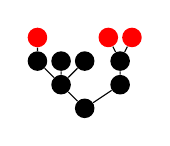
\begin{tikzpicture}[scale=.2]
\node[circle, scale=0.75, fill] (tid0) at (3.75,1.5){};
\node[circle, scale=0.75, fill] (tid1) at (2.25,3){};
\node[circle, scale=0.75, fill] (tid3) at (0.75,4.5){};
\node[circle, scale=0.75, fill, red] (tid7) at (0.75,6){};
\draw[](tid3) -- (tid7);
\node[circle, scale=0.75, fill] (tid4) at (2.25,4.5){};
\node[circle, scale=0.75, fill] (tid5) at (3.75,4.5){};
\draw[](tid1) -- (tid3);
\draw[](tid1) -- (tid4);
\draw[](tid1) -- (tid5);
\node[circle, scale=0.75, fill] (tid2) at (6,3){};
\node[circle, scale=0.75, fill] (tid6) at (6,4.5){};
\node[circle, scale=0.75, fill, red] (tid8) at (5.25,6){};
\node[circle, scale=0.75, fill, red] (tid9) at (6.75,6){};
\draw[](tid6) -- (tid8);
\draw[](tid6) -- (tid9);
\draw[](tid2) -- (tid6);
\draw[](tid0) -- (tid1);
\draw[](tid0) -- (tid2);
\end{tikzpicture}
\nodepart{two}
\footnotesize{5.60434}
\nodepart{three}
\footnotesize{$33\:67$}
};
 & 
\\
};
\end{scope}
\begin{scope}[yshift=\leveltopIII cm]
\matrix (line3) [column sep=1cm] {
\node[draw=black, rectangle split,  rectangle split parts=3] (sn0xd31f80){
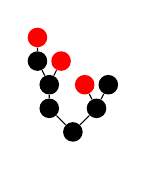
\begin{tikzpicture}[scale=.2]
\node[circle, scale=0.75, fill] (tid0) at (3,1.5){};
\node[circle, scale=0.75, fill] (tid1) at (1.5,3){};
\node[circle, scale=0.75, fill] (tid3) at (1.5,4.5){};
\node[circle, scale=0.75, fill] (tid6) at (0.75,6){};
\node[circle, scale=0.75, fill, red] (tid8) at (0.75,7.5){};
\draw[](tid6) -- (tid8);
\node[circle, scale=0.75, fill, red] (tid7) at (2.25,6){};
\draw[](tid3) -- (tid6);
\draw[](tid3) -- (tid7);
\draw[](tid1) -- (tid3);
\node[circle, scale=0.75, fill] (tid2) at (4.5,3){};
\node[circle, scale=0.75, fill, red] (tid4) at (3.75,4.5){};
\node[circle, scale=0.75, fill] (tid5) at (5.25,4.5){};
\draw[](tid2) -- (tid4);
\draw[](tid2) -- (tid5);
\draw[](tid0) -- (tid1);
\draw[](tid0) -- (tid2);
\end{tikzpicture}
\nodepart{two}
\footnotesize{5.62423}
\nodepart{three}
\footnotesize{$33\:33\:33$}
};
 & 
\node[draw=black, rectangle split,  rectangle split parts=3] (sn0xd32bc0){
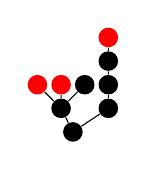
\begin{tikzpicture}[scale=.2]
\node[circle, scale=0.75, fill] (tid0) at (3,1.5){};
\node[circle, scale=0.75, fill] (tid1) at (2.25,3){};
\node[circle, scale=0.75, fill, red] (tid3) at (0.75,4.5){};
\node[circle, scale=0.75, fill, red] (tid4) at (2.25,4.5){};
\node[circle, scale=0.75, fill] (tid5) at (3.75,4.5){};
\draw[](tid1) -- (tid3);
\draw[](tid1) -- (tid4);
\draw[](tid1) -- (tid5);
\node[circle, scale=0.75, fill] (tid2) at (5.25,3){};
\node[circle, scale=0.75, fill] (tid6) at (5.25,4.5){};
\node[circle, scale=0.75, fill] (tid7) at (5.25,6){};
\node[circle, scale=0.75, fill, red] (tid8) at (5.25,7.5){};
\draw[](tid7) -- (tid8);
\draw[](tid6) -- (tid7);
\draw[](tid2) -- (tid6);
\draw[](tid0) -- (tid1);
\draw[](tid0) -- (tid2);
\end{tikzpicture}
\nodepart{two}
\footnotesize{5.55041}
\nodepart{three}
\footnotesize{$67\:33$}
};
 & 
\node[draw=black, rectangle split,  rectangle split parts=3] (sn0xd32890){
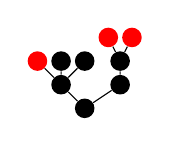
\begin{tikzpicture}[scale=.2]
\node[circle, scale=0.75, fill] (tid0) at (3.75,1.5){};
\node[circle, scale=0.75, fill] (tid1) at (2.25,3){};
\node[circle, scale=0.75, fill, red] (tid3) at (0.75,4.5){};
\node[circle, scale=0.75, fill] (tid4) at (2.25,4.5){};
\node[circle, scale=0.75, fill] (tid5) at (3.75,4.5){};
\draw[](tid1) -- (tid3);
\draw[](tid1) -- (tid4);
\draw[](tid1) -- (tid5);
\node[circle, scale=0.75, fill] (tid2) at (6,3){};
\node[circle, scale=0.75, fill] (tid6) at (6,4.5){};
\node[circle, scale=0.75, fill, red] (tid7) at (5.25,6){};
\node[circle, scale=0.75, fill, red] (tid8) at (6.75,6){};
\draw[](tid6) -- (tid7);
\draw[](tid6) -- (tid8);
\draw[](tid2) -- (tid6);
\draw[](tid0) -- (tid1);
\draw[](tid0) -- (tid2);
\end{tikzpicture}
\nodepart{two}
\footnotesize{5.27109}
\nodepart{three}
\footnotesize{$33\:67$}
};
 & 
\node[draw=black, rectangle split,  rectangle split parts=3] (sn0xd39c80){
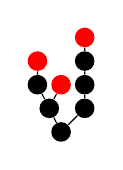
\begin{tikzpicture}[scale=.2]
\node[circle, scale=0.75, fill] (tid0) at (2.25,1.5){};
\node[circle, scale=0.75, fill] (tid1) at (1.5,3){};
\node[circle, scale=0.75, fill] (tid3) at (0.75,4.5){};
\node[circle, scale=0.75, fill, red] (tid6) at (0.75,6){};
\draw[](tid3) -- (tid6);
\node[circle, scale=0.75, fill, red] (tid4) at (2.25,4.5){};
\draw[](tid1) -- (tid3);
\draw[](tid1) -- (tid4);
\node[circle, scale=0.75, fill] (tid2) at (3.75,3){};
\node[circle, scale=0.75, fill] (tid5) at (3.75,4.5){};
\node[circle, scale=0.75, fill] (tid7) at (3.75,6){};
\node[circle, scale=0.75, fill, red] (tid8) at (3.75,7.5){};
\draw[](tid7) -- (tid8);
\draw[](tid5) -- (tid7);
\draw[](tid2) -- (tid5);
\draw[](tid0) -- (tid1);
\draw[](tid0) -- (tid2);
\end{tikzpicture}
\nodepart{two}
\footnotesize{5.67991}
\nodepart{three}
\footnotesize{$33\:33\:33$}
};
 & 
\node[draw=black, rectangle split,  rectangle split parts=3] (sn0xd393e0){
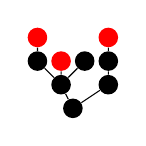
\begin{tikzpicture}[scale=.2]
\node[circle, scale=0.75, fill] (tid0) at (3,1.5){};
\node[circle, scale=0.75, fill] (tid1) at (2.25,3){};
\node[circle, scale=0.75, fill] (tid3) at (0.75,4.5){};
\node[circle, scale=0.75, fill, red] (tid7) at (0.75,6){};
\draw[](tid3) -- (tid7);
\node[circle, scale=0.75, fill, red] (tid4) at (2.25,4.5){};
\node[circle, scale=0.75, fill] (tid5) at (3.75,4.5){};
\draw[](tid1) -- (tid3);
\draw[](tid1) -- (tid4);
\draw[](tid1) -- (tid5);
\node[circle, scale=0.75, fill] (tid2) at (5.25,3){};
\node[circle, scale=0.75, fill] (tid6) at (5.25,4.5){};
\node[circle, scale=0.75, fill, red] (tid8) at (5.25,6){};
\draw[](tid6) -- (tid8);
\draw[](tid2) -- (tid6);
\draw[](tid0) -- (tid1);
\draw[](tid0) -- (tid2);
\end{tikzpicture}
\nodepart{two}
\footnotesize{5.27096}
\nodepart{three}
\footnotesize{$33\:33\:17\:17$}
};
 & 
\\
};
\end{scope}
\begin{scope}[yshift=\leveltopIIII cm]
\matrix (line4) [column sep=1cm] {
\node[draw=black, rectangle split,  rectangle split parts=3] (sn0xd2f660){
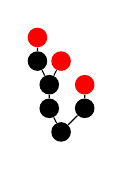
\begin{tikzpicture}[scale=.2]
\node[circle, scale=0.75, fill] (tid0) at (2.25,1.5){};
\node[circle, scale=0.75, fill] (tid1) at (1.5,3){};
\node[circle, scale=0.75, fill] (tid3) at (1.5,4.5){};
\node[circle, scale=0.75, fill] (tid5) at (0.75,6){};
\node[circle, scale=0.75, fill, red] (tid7) at (0.75,7.5){};
\draw[](tid5) -- (tid7);
\node[circle, scale=0.75, fill, red] (tid6) at (2.25,6){};
\draw[](tid3) -- (tid5);
\draw[](tid3) -- (tid6);
\draw[](tid1) -- (tid3);
\node[circle, scale=0.75, fill] (tid2) at (3.75,3){};
\node[circle, scale=0.75, fill, red] (tid4) at (3.75,4.5){};
\draw[](tid2) -- (tid4);
\draw[](tid0) -- (tid1);
\draw[](tid0) -- (tid2);
\end{tikzpicture}
\nodepart{two}
\footnotesize{5.45602}
\nodepart{three}
\footnotesize{$33\:33\:33$}
};
 & 
\node[draw=black, rectangle split,  rectangle split parts=3] (sn0xd32d10){
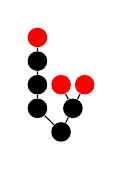
\begin{tikzpicture}[scale=.2]
\node[circle, scale=0.75, fill] (tid0) at (2.25,1.5){};
\node[circle, scale=0.75, fill] (tid1) at (0.75,3){};
\node[circle, scale=0.75, fill] (tid3) at (0.75,4.5){};
\node[circle, scale=0.75, fill] (tid6) at (0.75,6){};
\node[circle, scale=0.75, fill, red] (tid7) at (0.75,7.5){};
\draw[](tid6) -- (tid7);
\draw[](tid3) -- (tid6);
\draw[](tid1) -- (tid3);
\node[circle, scale=0.75, fill] (tid2) at (3,3){};
\node[circle, scale=0.75, fill, red] (tid4) at (2.25,4.5){};
\node[circle, scale=0.75, fill, red] (tid5) at (3.75,4.5){};
\draw[](tid2) -- (tid4);
\draw[](tid2) -- (tid5);
\draw[](tid0) -- (tid1);
\draw[](tid0) -- (tid2);
\end{tikzpicture}
\nodepart{two}
\footnotesize{5.38117}
\nodepart{three}
\footnotesize{$67\:33$}
};
 & 
\node[draw=black, rectangle split,  rectangle split parts=3] (sn0xd33760){
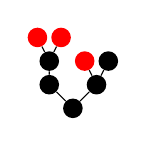
\begin{tikzpicture}[scale=.2]
\node[circle, scale=0.75, fill] (tid0) at (3,1.5){};
\node[circle, scale=0.75, fill] (tid1) at (1.5,3){};
\node[circle, scale=0.75, fill] (tid3) at (1.5,4.5){};
\node[circle, scale=0.75, fill, red] (tid6) at (0.75,6){};
\node[circle, scale=0.75, fill, red] (tid7) at (2.25,6){};
\draw[](tid3) -- (tid6);
\draw[](tid3) -- (tid7);
\draw[](tid1) -- (tid3);
\node[circle, scale=0.75, fill] (tid2) at (4.5,3){};
\node[circle, scale=0.75, fill, red] (tid4) at (3.75,4.5){};
\node[circle, scale=0.75, fill] (tid5) at (5.25,4.5){};
\draw[](tid2) -- (tid4);
\draw[](tid2) -- (tid5);
\draw[](tid0) -- (tid1);
\draw[](tid0) -- (tid2);
\end{tikzpicture}
\nodepart{two}
\footnotesize{5.03549}
\nodepart{three}
\footnotesize{$33\:67$}
};
 & 
\node[draw=black, rectangle split,  rectangle split parts=3] (sn0xd38b30){
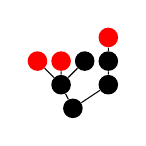
\begin{tikzpicture}[scale=.2]
\node[circle, scale=0.75, fill] (tid0) at (3,1.5){};
\node[circle, scale=0.75, fill] (tid1) at (2.25,3){};
\node[circle, scale=0.75, fill, red] (tid3) at (0.75,4.5){};
\node[circle, scale=0.75, fill, red] (tid4) at (2.25,4.5){};
\node[circle, scale=0.75, fill] (tid5) at (3.75,4.5){};
\draw[](tid1) -- (tid3);
\draw[](tid1) -- (tid4);
\draw[](tid1) -- (tid5);
\node[circle, scale=0.75, fill] (tid2) at (5.25,3){};
\node[circle, scale=0.75, fill] (tid6) at (5.25,4.5){};
\node[circle, scale=0.75, fill, red] (tid7) at (5.25,6){};
\draw[](tid6) -- (tid7);
\draw[](tid2) -- (tid6);
\draw[](tid0) -- (tid1);
\draw[](tid0) -- (tid2);
\end{tikzpicture}
\nodepart{two}
\footnotesize{4.88889}
\nodepart{three}
\footnotesize{$67\:17\:17$}
};
 & 
\node[draw=black, rectangle split,  rectangle split parts=3] (sn0xd3a540){
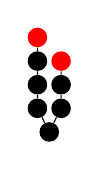
\begin{tikzpicture}[scale=.2]
\node[circle, scale=0.75, fill] (tid0) at (1.5,1.5){};
\node[circle, scale=0.75, fill] (tid1) at (0.75,3){};
\node[circle, scale=0.75, fill] (tid3) at (0.75,4.5){};
\node[circle, scale=0.75, fill] (tid5) at (0.75,6){};
\node[circle, scale=0.75, fill, red] (tid7) at (0.75,7.5){};
\draw[](tid5) -- (tid7);
\draw[](tid3) -- (tid5);
\draw[](tid1) -- (tid3);
\node[circle, scale=0.75, fill] (tid2) at (2.25,3){};
\node[circle, scale=0.75, fill] (tid4) at (2.25,4.5){};
\node[circle, scale=0.75, fill, red] (tid6) at (2.25,6){};
\draw[](tid4) -- (tid6);
\draw[](tid2) -- (tid4);
\draw[](tid0) -- (tid1);
\draw[](tid0) -- (tid2);
\end{tikzpicture}
\nodepart{two}
\footnotesize{5.59375}
\nodepart{three}
\footnotesize{$50\:50$}
};
 & 
\node[draw=black, rectangle split,  rectangle split parts=3] (sn0xd3aa20){
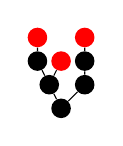
\begin{tikzpicture}[scale=.2]
\node[circle, scale=0.75, fill] (tid0) at (2.25,1.5){};
\node[circle, scale=0.75, fill] (tid1) at (1.5,3){};
\node[circle, scale=0.75, fill] (tid3) at (0.75,4.5){};
\node[circle, scale=0.75, fill, red] (tid6) at (0.75,6){};
\draw[](tid3) -- (tid6);
\node[circle, scale=0.75, fill, red] (tid4) at (2.25,4.5){};
\draw[](tid1) -- (tid3);
\draw[](tid1) -- (tid4);
\node[circle, scale=0.75, fill] (tid2) at (3.75,3){};
\node[circle, scale=0.75, fill] (tid5) at (3.75,4.5){};
\node[circle, scale=0.75, fill, red] (tid7) at (3.75,6){};
\draw[](tid5) -- (tid7);
\draw[](tid2) -- (tid5);
\draw[](tid0) -- (tid1);
\draw[](tid0) -- (tid2);
\end{tikzpicture}
\nodepart{two}
\footnotesize{5.06482}
\nodepart{three}
\footnotesize{$33\:33\:33$}
};
 & 
\node[draw=black, rectangle split,  rectangle split parts=3] (sn0xd3ba90){
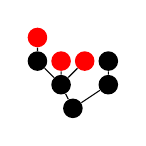
\begin{tikzpicture}[scale=.2]
\node[circle, scale=0.75, fill] (tid0) at (3,1.5){};
\node[circle, scale=0.75, fill] (tid1) at (2.25,3){};
\node[circle, scale=0.75, fill] (tid3) at (0.75,4.5){};
\node[circle, scale=0.75, fill, red] (tid7) at (0.75,6){};
\draw[](tid3) -- (tid7);
\node[circle, scale=0.75, fill, red] (tid4) at (2.25,4.5){};
\node[circle, scale=0.75, fill, red] (tid5) at (3.75,4.5){};
\draw[](tid1) -- (tid3);
\draw[](tid1) -- (tid4);
\draw[](tid1) -- (tid5);
\node[circle, scale=0.75, fill] (tid2) at (5.25,3){};
\node[circle, scale=0.75, fill] (tid6) at (5.25,4.5){};
\draw[](tid2) -- (tid6);
\draw[](tid0) -- (tid1);
\draw[](tid0) -- (tid2);
\end{tikzpicture}
\nodepart{two}
\footnotesize{4.86883}
\nodepart{three}
\footnotesize{$17\:17\:67$}
};
 & 
\node[draw=black, rectangle split,  rectangle split parts=3] (sn0xd3b560){
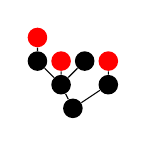
\begin{tikzpicture}[scale=.2]
\node[circle, scale=0.75, fill] (tid0) at (3,1.5){};
\node[circle, scale=0.75, fill] (tid1) at (2.25,3){};
\node[circle, scale=0.75, fill] (tid3) at (0.75,4.5){};
\node[circle, scale=0.75, fill, red] (tid7) at (0.75,6){};
\draw[](tid3) -- (tid7);
\node[circle, scale=0.75, fill, red] (tid4) at (2.25,4.5){};
\node[circle, scale=0.75, fill] (tid5) at (3.75,4.5){};
\draw[](tid1) -- (tid3);
\draw[](tid1) -- (tid4);
\draw[](tid1) -- (tid5);
\node[circle, scale=0.75, fill] (tid2) at (5.25,3){};
\node[circle, scale=0.75, fill, red] (tid6) at (5.25,4.5){};
\draw[](tid2) -- (tid6);
\draw[](tid0) -- (tid1);
\draw[](tid0) -- (tid2);
\end{tikzpicture}
\nodepart{two}
\footnotesize{4.84954}
\nodepart{three}
\footnotesize{$33\:33\:33$}
};
 & 
\\
};
\end{scope}
\begin{scope}[yshift=\leveltopIIIII cm]
\matrix (line5) [column sep=1cm] {
\node[draw=black, rectangle split,  rectangle split parts=3] (sn0xd33af0){
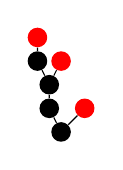
\begin{tikzpicture}[scale=.2]
\node[circle, scale=0.75, fill] (tid0) at (2.25,1.5){};
\node[circle, scale=0.75, fill] (tid1) at (1.5,3){};
\node[circle, scale=0.75, fill] (tid3) at (1.5,4.5){};
\node[circle, scale=0.75, fill] (tid4) at (0.75,6){};
\node[circle, scale=0.75, fill, red] (tid6) at (0.75,7.5){};
\draw[](tid4) -- (tid6);
\node[circle, scale=0.75, fill, red] (tid5) at (2.25,6){};
\draw[](tid3) -- (tid4);
\draw[](tid3) -- (tid5);
\draw[](tid1) -- (tid3);
\node[circle, scale=0.75, fill, red] (tid2) at (3.75,3){};
\draw[](tid0) -- (tid1);
\draw[](tid0) -- (tid2);
\end{tikzpicture}
\nodepart{two}
\footnotesize{5.29861}
\nodepart{three}
\footnotesize{$33\:33\:33$}
};
 & 
\node[draw=black, rectangle split,  rectangle split parts=3] (sn0xd32e50){
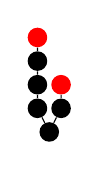
\begin{tikzpicture}[scale=.2]
\node[circle, scale=0.75, fill] (tid0) at (1.5,1.5){};
\node[circle, scale=0.75, fill] (tid1) at (0.75,3){};
\node[circle, scale=0.75, fill] (tid3) at (0.75,4.5){};
\node[circle, scale=0.75, fill] (tid5) at (0.75,6){};
\node[circle, scale=0.75, fill, red] (tid6) at (0.75,7.5){};
\draw[](tid5) -- (tid6);
\draw[](tid3) -- (tid5);
\draw[](tid1) -- (tid3);
\node[circle, scale=0.75, fill] (tid2) at (2.25,3){};
\node[circle, scale=0.75, fill, red] (tid4) at (2.25,4.5){};
\draw[](tid2) -- (tid4);
\draw[](tid0) -- (tid1);
\draw[](tid0) -- (tid2);
\end{tikzpicture}
\nodepart{two}
\footnotesize{5.25}
\nodepart{three}
\footnotesize{$50\:50$}
};
 & 
\node[draw=black, rectangle split,  rectangle split parts=3] (sn0xd33f60){
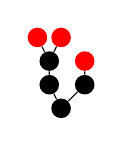
\begin{tikzpicture}[scale=.2]
\node[circle, scale=0.75, fill] (tid0) at (2.25,1.5){};
\node[circle, scale=0.75, fill] (tid1) at (1.5,3){};
\node[circle, scale=0.75, fill] (tid3) at (1.5,4.5){};
\node[circle, scale=0.75, fill, red] (tid5) at (0.75,6){};
\node[circle, scale=0.75, fill, red] (tid6) at (2.25,6){};
\draw[](tid3) -- (tid5);
\draw[](tid3) -- (tid6);
\draw[](tid1) -- (tid3);
\node[circle, scale=0.75, fill] (tid2) at (3.75,3){};
\node[circle, scale=0.75, fill, red] (tid4) at (3.75,4.5){};
\draw[](tid2) -- (tid4);
\draw[](tid0) -- (tid1);
\draw[](tid0) -- (tid2);
\end{tikzpicture}
\nodepart{two}
\footnotesize{4.81944}
\nodepart{three}
\footnotesize{$33\:67$}
};
 & 
\node[draw=black, rectangle split,  rectangle split parts=3] (sn0xd374a0){
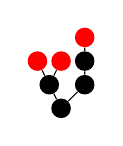
\begin{tikzpicture}[scale=.2]
\node[circle, scale=0.75, fill] (tid0) at (2.25,1.5){};
\node[circle, scale=0.75, fill] (tid1) at (1.5,3){};
\node[circle, scale=0.75, fill, red] (tid3) at (0.75,4.5){};
\node[circle, scale=0.75, fill, red] (tid4) at (2.25,4.5){};
\draw[](tid1) -- (tid3);
\draw[](tid1) -- (tid4);
\node[circle, scale=0.75, fill] (tid2) at (3.75,3){};
\node[circle, scale=0.75, fill] (tid5) at (3.75,4.5){};
\node[circle, scale=0.75, fill, red] (tid6) at (3.75,6){};
\draw[](tid5) -- (tid6);
\draw[](tid2) -- (tid5);
\draw[](tid0) -- (tid1);
\draw[](tid0) -- (tid2);
\end{tikzpicture}
\nodepart{two}
\footnotesize{4.64352}
\nodepart{three}
\footnotesize{$67\:33$}
};
 & 
\node[draw=black, rectangle split,  rectangle split parts=3] (sn0xd38a40){
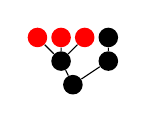
\begin{tikzpicture}[scale=.2]
\node[circle, scale=0.75, fill] (tid0) at (3,1.5){};
\node[circle, scale=0.75, fill] (tid1) at (2.25,3){};
\node[circle, scale=0.75, fill, red] (tid3) at (0.75,4.5){};
\node[circle, scale=0.75, fill, red] (tid4) at (2.25,4.5){};
\node[circle, scale=0.75, fill, red] (tid5) at (3.75,4.5){};
\draw[](tid1) -- (tid3);
\draw[](tid1) -- (tid4);
\draw[](tid1) -- (tid5);
\node[circle, scale=0.75, fill] (tid2) at (5.25,3){};
\node[circle, scale=0.75, fill] (tid6) at (5.25,4.5){};
\draw[](tid2) -- (tid6);
\draw[](tid0) -- (tid1);
\draw[](tid0) -- (tid2);
\end{tikzpicture}
\nodepart{two}
\footnotesize{4.38889}
\nodepart{three}
\footnotesize{$1$}
};
 & 
\node[draw=black, rectangle split,  rectangle split parts=3] (sn0xd38f70){
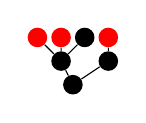
\begin{tikzpicture}[scale=.2]
\node[circle, scale=0.75, fill] (tid0) at (3,1.5){};
\node[circle, scale=0.75, fill] (tid1) at (2.25,3){};
\node[circle, scale=0.75, fill, red] (tid3) at (0.75,4.5){};
\node[circle, scale=0.75, fill, red] (tid4) at (2.25,4.5){};
\node[circle, scale=0.75, fill] (tid5) at (3.75,4.5){};
\draw[](tid1) -- (tid3);
\draw[](tid1) -- (tid4);
\draw[](tid1) -- (tid5);
\node[circle, scale=0.75, fill] (tid2) at (5.25,3){};
\node[circle, scale=0.75, fill, red] (tid6) at (5.25,4.5){};
\draw[](tid2) -- (tid6);
\draw[](tid0) -- (tid1);
\draw[](tid0) -- (tid2);
\end{tikzpicture}
\nodepart{two}
\footnotesize{4.37037}
\nodepart{three}
\footnotesize{$67\:33$}
};
 & 
\node[draw=black, rectangle split,  rectangle split parts=3] (sn0xd3ae10){
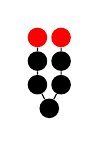
\begin{tikzpicture}[scale=.2]
\node[circle, scale=0.75, fill] (tid0) at (1.5,1.5){};
\node[circle, scale=0.75, fill] (tid1) at (0.75,3){};
\node[circle, scale=0.75, fill] (tid3) at (0.75,4.5){};
\node[circle, scale=0.75, fill, red] (tid5) at (0.75,6){};
\draw[](tid3) -- (tid5);
\draw[](tid1) -- (tid3);
\node[circle, scale=0.75, fill] (tid2) at (2.25,3){};
\node[circle, scale=0.75, fill] (tid4) at (2.25,4.5){};
\node[circle, scale=0.75, fill, red] (tid6) at (2.25,6){};
\draw[](tid4) -- (tid6);
\draw[](tid2) -- (tid4);
\draw[](tid0) -- (tid1);
\draw[](tid0) -- (tid2);
\end{tikzpicture}
\nodepart{two}
\footnotesize{4.9375}
\nodepart{three}
\footnotesize{$1$}
};
 & 
\node[draw=black, rectangle split,  rectangle split parts=3] (sn0xd3b0e0){
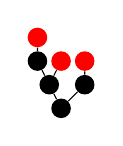
\begin{tikzpicture}[scale=.2]
\node[circle, scale=0.75, fill] (tid0) at (2.25,1.5){};
\node[circle, scale=0.75, fill] (tid1) at (1.5,3){};
\node[circle, scale=0.75, fill] (tid3) at (0.75,4.5){};
\node[circle, scale=0.75, fill, red] (tid6) at (0.75,6){};
\draw[](tid3) -- (tid6);
\node[circle, scale=0.75, fill, red] (tid4) at (2.25,4.5){};
\draw[](tid1) -- (tid3);
\draw[](tid1) -- (tid4);
\node[circle, scale=0.75, fill] (tid2) at (3.75,3){};
\node[circle, scale=0.75, fill, red] (tid5) at (3.75,4.5){};
\draw[](tid2) -- (tid5);
\draw[](tid0) -- (tid1);
\draw[](tid0) -- (tid2);
\end{tikzpicture}
\nodepart{two}
\footnotesize{4.61343}
\nodepart{three}
\footnotesize{$33\:33\:33$}
};
 & 
\node[draw=black, rectangle split,  rectangle split parts=3] (sn0xd3ca90){
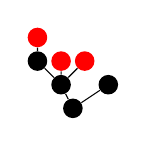
\begin{tikzpicture}[scale=.2]
\node[circle, scale=0.75, fill] (tid0) at (3,1.5){};
\node[circle, scale=0.75, fill] (tid1) at (2.25,3){};
\node[circle, scale=0.75, fill] (tid3) at (0.75,4.5){};
\node[circle, scale=0.75, fill, red] (tid6) at (0.75,6){};
\draw[](tid3) -- (tid6);
\node[circle, scale=0.75, fill, red] (tid4) at (2.25,4.5){};
\node[circle, scale=0.75, fill, red] (tid5) at (3.75,4.5){};
\draw[](tid1) -- (tid3);
\draw[](tid1) -- (tid4);
\draw[](tid1) -- (tid5);
\node[circle, scale=0.75, fill] (tid2) at (5.25,3){};
\draw[](tid0) -- (tid1);
\draw[](tid0) -- (tid2);
\end{tikzpicture}
\nodepart{two}
\footnotesize{4.56482}
\nodepart{three}
\footnotesize{$33\:67$}
};
 & 
\\
};
\end{scope}
\begin{scope}[yshift=\leveltopIIIIII cm]
\matrix (line6) [column sep=1cm] {
\node[draw=black, rectangle split,  rectangle split parts=3] (sn0xd345e0){
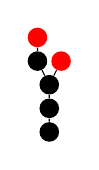
\begin{tikzpicture}[scale=.2]
\node[circle, scale=0.75, fill] (tid0) at (1.5,1.5){};
\node[circle, scale=0.75, fill] (tid1) at (1.5,3){};
\node[circle, scale=0.75, fill] (tid2) at (1.5,4.5){};
\node[circle, scale=0.75, fill] (tid3) at (0.75,6){};
\node[circle, scale=0.75, fill, red] (tid5) at (0.75,7.5){};
\draw[](tid3) -- (tid5);
\node[circle, scale=0.75, fill, red] (tid4) at (2.25,6){};
\draw[](tid2) -- (tid3);
\draw[](tid2) -- (tid4);
\draw[](tid1) -- (tid2);
\draw[](tid0) -- (tid1);
\end{tikzpicture}
\nodepart{two}
\footnotesize{5.25}
\nodepart{three}
\footnotesize{$50\:50$}
};
 & 
\node[draw=black, rectangle split,  rectangle split parts=3] (sn0xd34350){
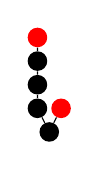
\begin{tikzpicture}[scale=.2]
\node[circle, scale=0.75, fill] (tid0) at (1.5,1.5){};
\node[circle, scale=0.75, fill] (tid1) at (0.75,3){};
\node[circle, scale=0.75, fill] (tid3) at (0.75,4.5){};
\node[circle, scale=0.75, fill] (tid4) at (0.75,6){};
\node[circle, scale=0.75, fill, red] (tid5) at (0.75,7.5){};
\draw[](tid4) -- (tid5);
\draw[](tid3) -- (tid4);
\draw[](tid1) -- (tid3);
\node[circle, scale=0.75, fill, red] (tid2) at (2.25,3){};
\draw[](tid0) -- (tid1);
\draw[](tid0) -- (tid2);
\end{tikzpicture}
\nodepart{two}
\footnotesize{5.0625}
\nodepart{three}
\footnotesize{$50\:50$}
};
 & 
\node[draw=black, rectangle split,  rectangle split parts=3] (sn0xd34410){
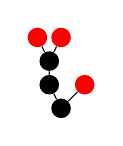
\begin{tikzpicture}[scale=.2]
\node[circle, scale=0.75, fill] (tid0) at (2.25,1.5){};
\node[circle, scale=0.75, fill] (tid1) at (1.5,3){};
\node[circle, scale=0.75, fill] (tid3) at (1.5,4.5){};
\node[circle, scale=0.75, fill, red] (tid4) at (0.75,6){};
\node[circle, scale=0.75, fill, red] (tid5) at (2.25,6){};
\draw[](tid3) -- (tid4);
\draw[](tid3) -- (tid5);
\draw[](tid1) -- (tid3);
\node[circle, scale=0.75, fill, red] (tid2) at (3.75,3){};
\draw[](tid0) -- (tid1);
\draw[](tid0) -- (tid2);
\end{tikzpicture}
\nodepart{two}
\footnotesize{4.58333}
\nodepart{three}
\footnotesize{$33\:67$}
};
 & 
\node[draw=black, rectangle split,  rectangle split parts=3] (sn0xd36a40){
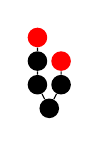
\begin{tikzpicture}[scale=.2]
\node[circle, scale=0.75, fill] (tid0) at (1.5,1.5){};
\node[circle, scale=0.75, fill] (tid1) at (0.75,3){};
\node[circle, scale=0.75, fill] (tid3) at (0.75,4.5){};
\node[circle, scale=0.75, fill, red] (tid5) at (0.75,6){};
\draw[](tid3) -- (tid5);
\draw[](tid1) -- (tid3);
\node[circle, scale=0.75, fill] (tid2) at (2.25,3){};
\node[circle, scale=0.75, fill, red] (tid4) at (2.25,4.5){};
\draw[](tid2) -- (tid4);
\draw[](tid0) -- (tid1);
\draw[](tid0) -- (tid2);
\end{tikzpicture}
\nodepart{two}
\footnotesize{4.4375}
\nodepart{three}
\footnotesize{$50\:50$}
};
 & 
\node[draw=black, rectangle split,  rectangle split parts=3] (sn0xd37280){
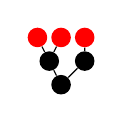
\begin{tikzpicture}[scale=.2]
\node[circle, scale=0.75, fill] (tid0) at (2.25,1.5){};
\node[circle, scale=0.75, fill] (tid1) at (1.5,3){};
\node[circle, scale=0.75, fill, red] (tid3) at (0.75,4.5){};
\node[circle, scale=0.75, fill, red] (tid4) at (2.25,4.5){};
\draw[](tid1) -- (tid3);
\draw[](tid1) -- (tid4);
\node[circle, scale=0.75, fill] (tid2) at (3.75,3){};
\node[circle, scale=0.75, fill, red] (tid5) at (3.75,4.5){};
\draw[](tid2) -- (tid5);
\draw[](tid0) -- (tid1);
\draw[](tid0) -- (tid2);
\end{tikzpicture}
\nodepart{two}
\footnotesize{4.05556}
\nodepart{three}
\footnotesize{$67\:33$}
};
 & 
\node[draw=black, rectangle split,  rectangle split parts=3] (sn0xd38090){
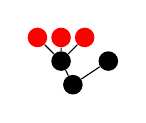
\begin{tikzpicture}[scale=.2]
\node[circle, scale=0.75, fill] (tid0) at (3,1.5){};
\node[circle, scale=0.75, fill] (tid1) at (2.25,3){};
\node[circle, scale=0.75, fill, red] (tid3) at (0.75,4.5){};
\node[circle, scale=0.75, fill, red] (tid4) at (2.25,4.5){};
\node[circle, scale=0.75, fill, red] (tid5) at (3.75,4.5){};
\draw[](tid1) -- (tid3);
\draw[](tid1) -- (tid4);
\draw[](tid1) -- (tid5);
\node[circle, scale=0.75, fill] (tid2) at (5.25,3){};
\draw[](tid0) -- (tid1);
\draw[](tid0) -- (tid2);
\end{tikzpicture}
\nodepart{two}
\footnotesize{4}
\nodepart{three}
\footnotesize{$1$}
};
 & 
\node[draw=black, rectangle split,  rectangle split parts=3] (sn0xd3aba0){
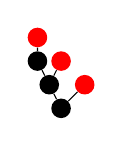
\begin{tikzpicture}[scale=.2]
\node[circle, scale=0.75, fill] (tid0) at (2.25,1.5){};
\node[circle, scale=0.75, fill] (tid1) at (1.5,3){};
\node[circle, scale=0.75, fill] (tid3) at (0.75,4.5){};
\node[circle, scale=0.75, fill, red] (tid5) at (0.75,6){};
\draw[](tid3) -- (tid5);
\node[circle, scale=0.75, fill, red] (tid4) at (2.25,4.5){};
\draw[](tid1) -- (tid3);
\draw[](tid1) -- (tid4);
\node[circle, scale=0.75, fill, red] (tid2) at (3.75,3){};
\draw[](tid0) -- (tid1);
\draw[](tid0) -- (tid2);
\end{tikzpicture}
\nodepart{two}
\footnotesize{4.34722}
\nodepart{three}
\footnotesize{$33\:33\:33$}
};
 & 
\\
};
\end{scope}
\begin{scope}[yshift=\leveltopIIIIIII cm]
\matrix (line7) [column sep=1cm] {
\node[draw=black, rectangle split,  rectangle split parts=3] (sn0xd35200){
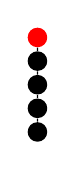
\begin{tikzpicture}[scale=.2]
\node[circle, scale=0.75, fill] (tid0) at (0.75,1.5){};
\node[circle, scale=0.75, fill] (tid1) at (0.75,3){};
\node[circle, scale=0.75, fill] (tid2) at (0.75,4.5){};
\node[circle, scale=0.75, fill] (tid3) at (0.75,6){};
\node[circle, scale=0.75, fill, red] (tid4) at (0.75,7.5){};
\draw[](tid3) -- (tid4);
\draw[](tid2) -- (tid3);
\draw[](tid1) -- (tid2);
\draw[](tid0) -- (tid1);
\end{tikzpicture}
\nodepart{two}
\footnotesize{5}
\nodepart{three}
\footnotesize{$1$}
};
 & 
\node[draw=black, rectangle split,  rectangle split parts=3] (sn0xd354a0){
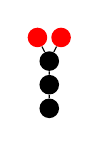
\begin{tikzpicture}[scale=.2]
\node[circle, scale=0.75, fill] (tid0) at (1.5,1.5){};
\node[circle, scale=0.75, fill] (tid1) at (1.5,3){};
\node[circle, scale=0.75, fill] (tid2) at (1.5,4.5){};
\node[circle, scale=0.75, fill, red] (tid3) at (0.75,6){};
\node[circle, scale=0.75, fill, red] (tid4) at (2.25,6){};
\draw[](tid2) -- (tid3);
\draw[](tid2) -- (tid4);
\draw[](tid1) -- (tid2);
\draw[](tid0) -- (tid1);
\end{tikzpicture}
\nodepart{two}
\footnotesize{4.5}
\nodepart{three}
\footnotesize{$1$}
};
 & 
\node[draw=black, rectangle split,  rectangle split parts=3] (sn0xd35c70){
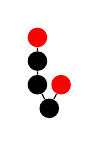
\begin{tikzpicture}[scale=.2]
\node[circle, scale=0.75, fill] (tid0) at (1.5,1.5){};
\node[circle, scale=0.75, fill] (tid1) at (0.75,3){};
\node[circle, scale=0.75, fill] (tid3) at (0.75,4.5){};
\node[circle, scale=0.75, fill, red] (tid4) at (0.75,6){};
\draw[](tid3) -- (tid4);
\draw[](tid1) -- (tid3);
\node[circle, scale=0.75, fill, red] (tid2) at (2.25,3){};
\draw[](tid0) -- (tid1);
\draw[](tid0) -- (tid2);
\end{tikzpicture}
\nodepart{two}
\footnotesize{4.125}
\nodepart{three}
\footnotesize{$50\:50$}
};
 & 
\node[draw=black, rectangle split,  rectangle split parts=3] (sn0xd37080){
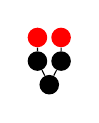
\begin{tikzpicture}[scale=.2]
\node[circle, scale=0.75, fill] (tid0) at (1.5,1.5){};
\node[circle, scale=0.75, fill] (tid1) at (0.75,3){};
\node[circle, scale=0.75, fill, red] (tid3) at (0.75,4.5){};
\draw[](tid1) -- (tid3);
\node[circle, scale=0.75, fill] (tid2) at (2.25,3){};
\node[circle, scale=0.75, fill, red] (tid4) at (2.25,4.5){};
\draw[](tid2) -- (tid4);
\draw[](tid0) -- (tid1);
\draw[](tid0) -- (tid2);
\end{tikzpicture}
\nodepart{two}
\footnotesize{3.75}
\nodepart{three}
\footnotesize{$1$}
};
 & 
\node[draw=black, rectangle split,  rectangle split parts=3] (sn0xd37c30){
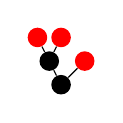
\begin{tikzpicture}[scale=.2]
\node[circle, scale=0.75, fill] (tid0) at (2.25,1.5){};
\node[circle, scale=0.75, fill] (tid1) at (1.5,3){};
\node[circle, scale=0.75, fill, red] (tid3) at (0.75,4.5){};
\node[circle, scale=0.75, fill, red] (tid4) at (2.25,4.5){};
\draw[](tid1) -- (tid3);
\draw[](tid1) -- (tid4);
\node[circle, scale=0.75, fill, red] (tid2) at (3.75,3){};
\draw[](tid0) -- (tid1);
\draw[](tid0) -- (tid2);
\end{tikzpicture}
\nodepart{two}
\footnotesize{3.66667}
\nodepart{three}
\footnotesize{$67\:33$}
};
 & 
\node[draw=black, rectangle split,  rectangle split parts=3] (sn0xd3b4a0){
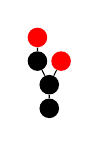
\begin{tikzpicture}[scale=.2]
\node[circle, scale=0.75, fill] (tid0) at (1.5,1.5){};
\node[circle, scale=0.75, fill] (tid1) at (1.5,3){};
\node[circle, scale=0.75, fill] (tid2) at (0.75,4.5){};
\node[circle, scale=0.75, fill, red] (tid4) at (0.75,6){};
\draw[](tid2) -- (tid4);
\node[circle, scale=0.75, fill, red] (tid3) at (2.25,4.5){};
\draw[](tid1) -- (tid2);
\draw[](tid1) -- (tid3);
\draw[](tid0) -- (tid1);
\end{tikzpicture}
\nodepart{two}
\footnotesize{4.25}
\nodepart{three}
\footnotesize{$50\:50$}
};
 & 
\\
};
\end{scope}
\begin{scope}[yshift=\leveltopIIIIIIII cm]
\matrix (line8) [column sep=1cm] {
\node[draw=black, rectangle split,  rectangle split parts=3] (sn0xd34c30){
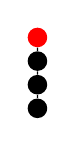
\begin{tikzpicture}[scale=.2]
\node[circle, scale=0.75, fill] (tid0) at (0.75,1.5){};
\node[circle, scale=0.75, fill] (tid1) at (0.75,3){};
\node[circle, scale=0.75, fill] (tid2) at (0.75,4.5){};
\node[circle, scale=0.75, fill, red] (tid3) at (0.75,6){};
\draw[](tid2) -- (tid3);
\draw[](tid1) -- (tid2);
\draw[](tid0) -- (tid1);
\end{tikzpicture}
\nodepart{two}
\footnotesize{4}
\nodepart{three}
\footnotesize{$1$}
};
 & 
\node[draw=black, rectangle split,  rectangle split parts=3] (sn0xd361a0){
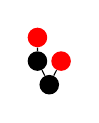
\begin{tikzpicture}[scale=.2]
\node[circle, scale=0.75, fill] (tid0) at (1.5,1.5){};
\node[circle, scale=0.75, fill] (tid1) at (0.75,3){};
\node[circle, scale=0.75, fill, red] (tid3) at (0.75,4.5){};
\draw[](tid1) -- (tid3);
\node[circle, scale=0.75, fill, red] (tid2) at (2.25,3){};
\draw[](tid0) -- (tid1);
\draw[](tid0) -- (tid2);
\end{tikzpicture}
\nodepart{two}
\footnotesize{3.25}
\nodepart{three}
\footnotesize{$50\:50$}
};
 & 
\node[draw=black, rectangle split,  rectangle split parts=3] (sn0xd375f0){
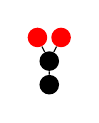
\begin{tikzpicture}[scale=.2]
\node[circle, scale=0.75, fill] (tid0) at (1.5,1.5){};
\node[circle, scale=0.75, fill] (tid1) at (1.5,3){};
\node[circle, scale=0.75, fill, red] (tid2) at (0.75,4.5){};
\node[circle, scale=0.75, fill, red] (tid3) at (2.25,4.5){};
\draw[](tid1) -- (tid2);
\draw[](tid1) -- (tid3);
\draw[](tid0) -- (tid1);
\end{tikzpicture}
\nodepart{two}
\footnotesize{3.5}
\nodepart{three}
\footnotesize{$1$}
};
 & 
\\
};
\end{scope}
\begin{scope}[yshift=\leveltopIIIIIIIII cm]
\matrix (line9) [column sep=1cm] {
\node[draw=black, rectangle split,  rectangle split parts=3] (sn0xd356c0){
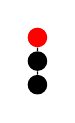
\begin{tikzpicture}[scale=.2]
\node[circle, scale=0.75, fill] (tid0) at (0.75,1.5){};
\node[circle, scale=0.75, fill] (tid1) at (0.75,3){};
\node[circle, scale=0.75, fill, red] (tid2) at (0.75,4.5){};
\draw[](tid1) -- (tid2);
\draw[](tid0) -- (tid1);
\end{tikzpicture}
\nodepart{two}
\footnotesize{3}
\nodepart{three}
\footnotesize{$1$}
};
 & 
\node[draw=black, rectangle split,  rectangle split parts=3] (sn0xd36020){

\begin{tikzpicture}[scale=.2]
\node[circle, scale=0.75, fill] (tid0) at (1.5,1.5){};
\node[circle, scale=0.75, fill, red] (tid1) at (0.75,3){};
\node[circle, scale=0.75, fill, red] (tid2) at (2.25,3){};
\draw[](tid0) -- (tid1);
\draw[](tid0) -- (tid2);
\end{tikzpicture}
\nodepart{two}
\footnotesize{2.5}
\nodepart{three}
\footnotesize{$1$}
};
 & 
\\
};
\end{scope}
\begin{scope}[yshift=\leveltopIIIIIIIIII cm]
\matrix (line10) [column sep=1cm] {
\node[draw=black, rectangle split,  rectangle split parts=3] (sn0xd34cf0){

\begin{tikzpicture}[scale=.2]
\node[circle, scale=0.75, fill] (tid0) at (0.75,1.5){};
\node[circle, scale=0.75, fill, red] (tid1) at (0.75,3){};
\draw[](tid0) -- (tid1);
\end{tikzpicture}
\nodepart{two}
\footnotesize{2}
\nodepart{three}
\footnotesize{$1$}
};
 & 
\\
};
\end{scope}
\begin{scope}[yshift=\leveltopIIIIIIIIIII cm]
\matrix (line11) [column sep=1cm] {
\node[draw=black, rectangle split,  rectangle split parts=3] (sn0xd35780){

\begin{tikzpicture}[scale=.2]
\node[circle, scale=0.75, fill, red] (tid0) at (0.75,1.5){};
\end{tikzpicture}
\nodepart{two}
\footnotesize{1}
\nodepart{three}
\footnotesize{$$}
};
 & 
\\
};
\end{scope}
\begin{scope}[yshift=\leveltopIIIIIIIIIIII cm]
\matrix (line12) [column sep=1cm] {
\\
};
\end{scope}
\draw (sn0xd2f280.south) -- (sn0xd31900.north);
\draw (sn0xd2f280.south) -- (sn0xd2e850.north);
\draw (sn0xd2f280.south) -- (sn0xd31a10.north);
\draw (sn0xd31900.south) -- (sn0xd31f80.north);
\draw (sn0xd31900.south) -- (sn0xd32bc0.north);
\draw (sn0xd31900.south) -- (sn0xd32890.north);
\draw (sn0xd2e850.south) -- (sn0xd39c80.north);
\draw (sn0xd2e850.south) -- (sn0xd32bc0.north);
\draw (sn0xd2e850.south) -- (sn0xd393e0.north);
\draw (sn0xd31a10.south) -- (sn0xd32890.north);
\draw (sn0xd31a10.south) -- (sn0xd393e0.north);
\draw (sn0xd31f80.south) -- (sn0xd2f660.north);
\draw (sn0xd31f80.south) -- (sn0xd32d10.north);
\draw (sn0xd31f80.south) -- (sn0xd33760.north);
\draw (sn0xd32bc0.south) -- (sn0xd32d10.north);
\draw (sn0xd32bc0.south) -- (sn0xd38b30.north);
\draw (sn0xd32890.south) -- (sn0xd33760.north);
\draw (sn0xd32890.south) -- (sn0xd38b30.north);
\draw (sn0xd39c80.south) -- (sn0xd3a540.north);
\draw (sn0xd39c80.south) -- (sn0xd32d10.north);
\draw (sn0xd39c80.south) -- (sn0xd3aa20.north);
\draw (sn0xd393e0.south) -- (sn0xd3aa20.north);
\draw (sn0xd393e0.south) -- (sn0xd38b30.north);
\draw (sn0xd393e0.south) -- (sn0xd3ba90.north);
\draw (sn0xd393e0.south) -- (sn0xd3b560.north);
\draw (sn0xd2f660.south) -- (sn0xd33af0.north);
\draw (sn0xd2f660.south) -- (sn0xd32e50.north);
\draw (sn0xd2f660.south) -- (sn0xd33f60.north);
\draw (sn0xd32d10.south) -- (sn0xd32e50.north);
\draw (sn0xd32d10.south) -- (sn0xd374a0.north);
\draw (sn0xd33760.south) -- (sn0xd33f60.north);
\draw (sn0xd33760.south) -- (sn0xd374a0.north);
\draw (sn0xd38b30.south) -- (sn0xd374a0.north);
\draw (sn0xd38b30.south) -- (sn0xd38a40.north);
\draw (sn0xd38b30.south) -- (sn0xd38f70.north);
\draw (sn0xd3a540.south) -- (sn0xd32e50.north);
\draw (sn0xd3a540.south) -- (sn0xd3ae10.north);
\draw (sn0xd3aa20.south) -- (sn0xd3ae10.north);
\draw (sn0xd3aa20.south) -- (sn0xd374a0.north);
\draw (sn0xd3aa20.south) -- (sn0xd3b0e0.north);
\draw (sn0xd3ba90.south) -- (sn0xd3b0e0.north);
\draw (sn0xd3ba90.south) -- (sn0xd38a40.north);
\draw (sn0xd3ba90.south) -- (sn0xd38f70.north);
\draw (sn0xd3b560.south) -- (sn0xd3b0e0.north);
\draw (sn0xd3b560.south) -- (sn0xd3ca90.north);
\draw (sn0xd3b560.south) -- (sn0xd38f70.north);
\draw (sn0xd33af0.south) -- (sn0xd345e0.north);
\draw (sn0xd33af0.south) -- (sn0xd34350.north);
\draw (sn0xd33af0.south) -- (sn0xd34410.north);
\draw (sn0xd32e50.south) -- (sn0xd34350.north);
\draw (sn0xd32e50.south) -- (sn0xd36a40.north);
\draw (sn0xd33f60.south) -- (sn0xd34410.north);
\draw (sn0xd33f60.south) -- (sn0xd36a40.north);
\draw (sn0xd374a0.south) -- (sn0xd36a40.north);
\draw (sn0xd374a0.south) -- (sn0xd37280.north);
\draw (sn0xd38a40.south) -- (sn0xd37280.north);
\draw (sn0xd38f70.south) -- (sn0xd37280.north);
\draw (sn0xd38f70.south) -- (sn0xd38090.north);
\draw (sn0xd3ae10.south) -- (sn0xd36a40.north);
\draw (sn0xd3b0e0.south) -- (sn0xd36a40.north);
\draw (sn0xd3b0e0.south) -- (sn0xd3aba0.north);
\draw (sn0xd3b0e0.south) -- (sn0xd37280.north);
\draw (sn0xd3ca90.south) -- (sn0xd3aba0.north);
\draw (sn0xd3ca90.south) -- (sn0xd38090.north);
\draw (sn0xd345e0.south) -- (sn0xd35200.north);
\draw (sn0xd345e0.south) -- (sn0xd354a0.north);
\draw (sn0xd34350.south) -- (sn0xd35200.north);
\draw (sn0xd34350.south) -- (sn0xd35c70.north);
\draw (sn0xd34410.south) -- (sn0xd354a0.north);
\draw (sn0xd34410.south) -- (sn0xd35c70.north);
\draw (sn0xd36a40.south) -- (sn0xd35c70.north);
\draw (sn0xd36a40.south) -- (sn0xd37080.north);
\draw (sn0xd37280.south) -- (sn0xd37080.north);
\draw (sn0xd37280.south) -- (sn0xd37c30.north);
\draw (sn0xd38090.south) -- (sn0xd37c30.north);
\draw (sn0xd3aba0.south) -- (sn0xd3b4a0.north);
\draw (sn0xd3aba0.south) -- (sn0xd35c70.north);
\draw (sn0xd3aba0.south) -- (sn0xd37c30.north);
\draw (sn0xd35200.south) -- (sn0xd34c30.north);
\draw (sn0xd354a0.south) -- (sn0xd34c30.north);
\draw (sn0xd35c70.south) -- (sn0xd34c30.north);
\draw (sn0xd35c70.south) -- (sn0xd361a0.north);
\draw (sn0xd37080.south) -- (sn0xd361a0.north);
\draw (sn0xd37c30.south) -- (sn0xd375f0.north);
\draw (sn0xd37c30.south) -- (sn0xd361a0.north);
\draw (sn0xd3b4a0.south) -- (sn0xd34c30.north);
\draw (sn0xd3b4a0.south) -- (sn0xd375f0.north);
\draw (sn0xd34c30.south) -- (sn0xd356c0.north);
\draw (sn0xd361a0.south) -- (sn0xd356c0.north);
\draw (sn0xd361a0.south) -- (sn0xd36020.north);
\draw (sn0xd375f0.south) -- (sn0xd356c0.north);
\draw (sn0xd356c0.south) -- (sn0xd34cf0.north);
\draw (sn0xd36020.south) -- (sn0xd34cf0.north);
\draw (sn0xd34cf0.south) -- (sn0xd35780.north);
\end{tikzpicture}

%%% Local Variables:
%%% TeX-master: "thesis/thesis.tex"
%%% End: 
